\documentclass[11pt]{article}

\usepackage[margin=1in]{geometry}
\usepackage{amsmath,amssymb}
\usepackage{booktabs}
\usepackage{graphicx}
\usepackage{float}
\usepackage{hyperref}
\usepackage{array}
\usepackage{longtable}
\usepackage{setspace}

\hypersetup{
  colorlinks=true,
  linkcolor=blue,
  urlcolor=blue,
  citecolor=blue
}

\title{From Reference Equations to Implemented Simulators:\\
An Explicit, Didactic Derivation for the VO\textsubscript{2} Single-Neuristor Project}
\author{Single-Neuristor Project Documentation}
\date{\today}

\begin{document}
\maketitle
\onehalfspacing

\begin{abstract}
This document provides a fully explicit, step-by-step scientific demonstration of the model implemented in this project. We start from what is \emph{known} from the two reference papers and from the experimental dataset, then derive the equations used in code, including the current-driven extension and the ideal-current-source limit. We then show how measured temperature--resistance data are transformed into hysteresis-related quantities, how parameters are fitted, and how the fitted model is validated against measured points. The objective is reproducibility and traceability: every mathematical object is defined, every assumption is stated, and every implemented step is connected to code modules and data artifacts.
\end{abstract}

\section{What We Know, and From Where}

\subsection{Primary sources of truth}
The project uses three primary information sources:

\begin{enumerate}
    \item \textbf{Thermal-neuristor dynamics paper (2024)}: Zhang \emph{et al.}, \emph{Nature Communications}, which provides the coupled electrical/thermal differential equations for VO\textsubscript{2} neuristors.
    \item \textbf{Hysteresis modeling paper (2002)}: de Almeida \emph{et al.}, \emph{Optical Engineering}, which provides the major/minor-loop hysteresis formalism used for \(R(T)\).
    \item \textbf{Experimental specimen data}: \texttt{data/experimental/100425\_chip1\_gap3.tsv}, containing measured temperature and resistance trajectories.
\end{enumerate}

\subsection{Lineage overview}
\begin{figure}[H]
    \centering
    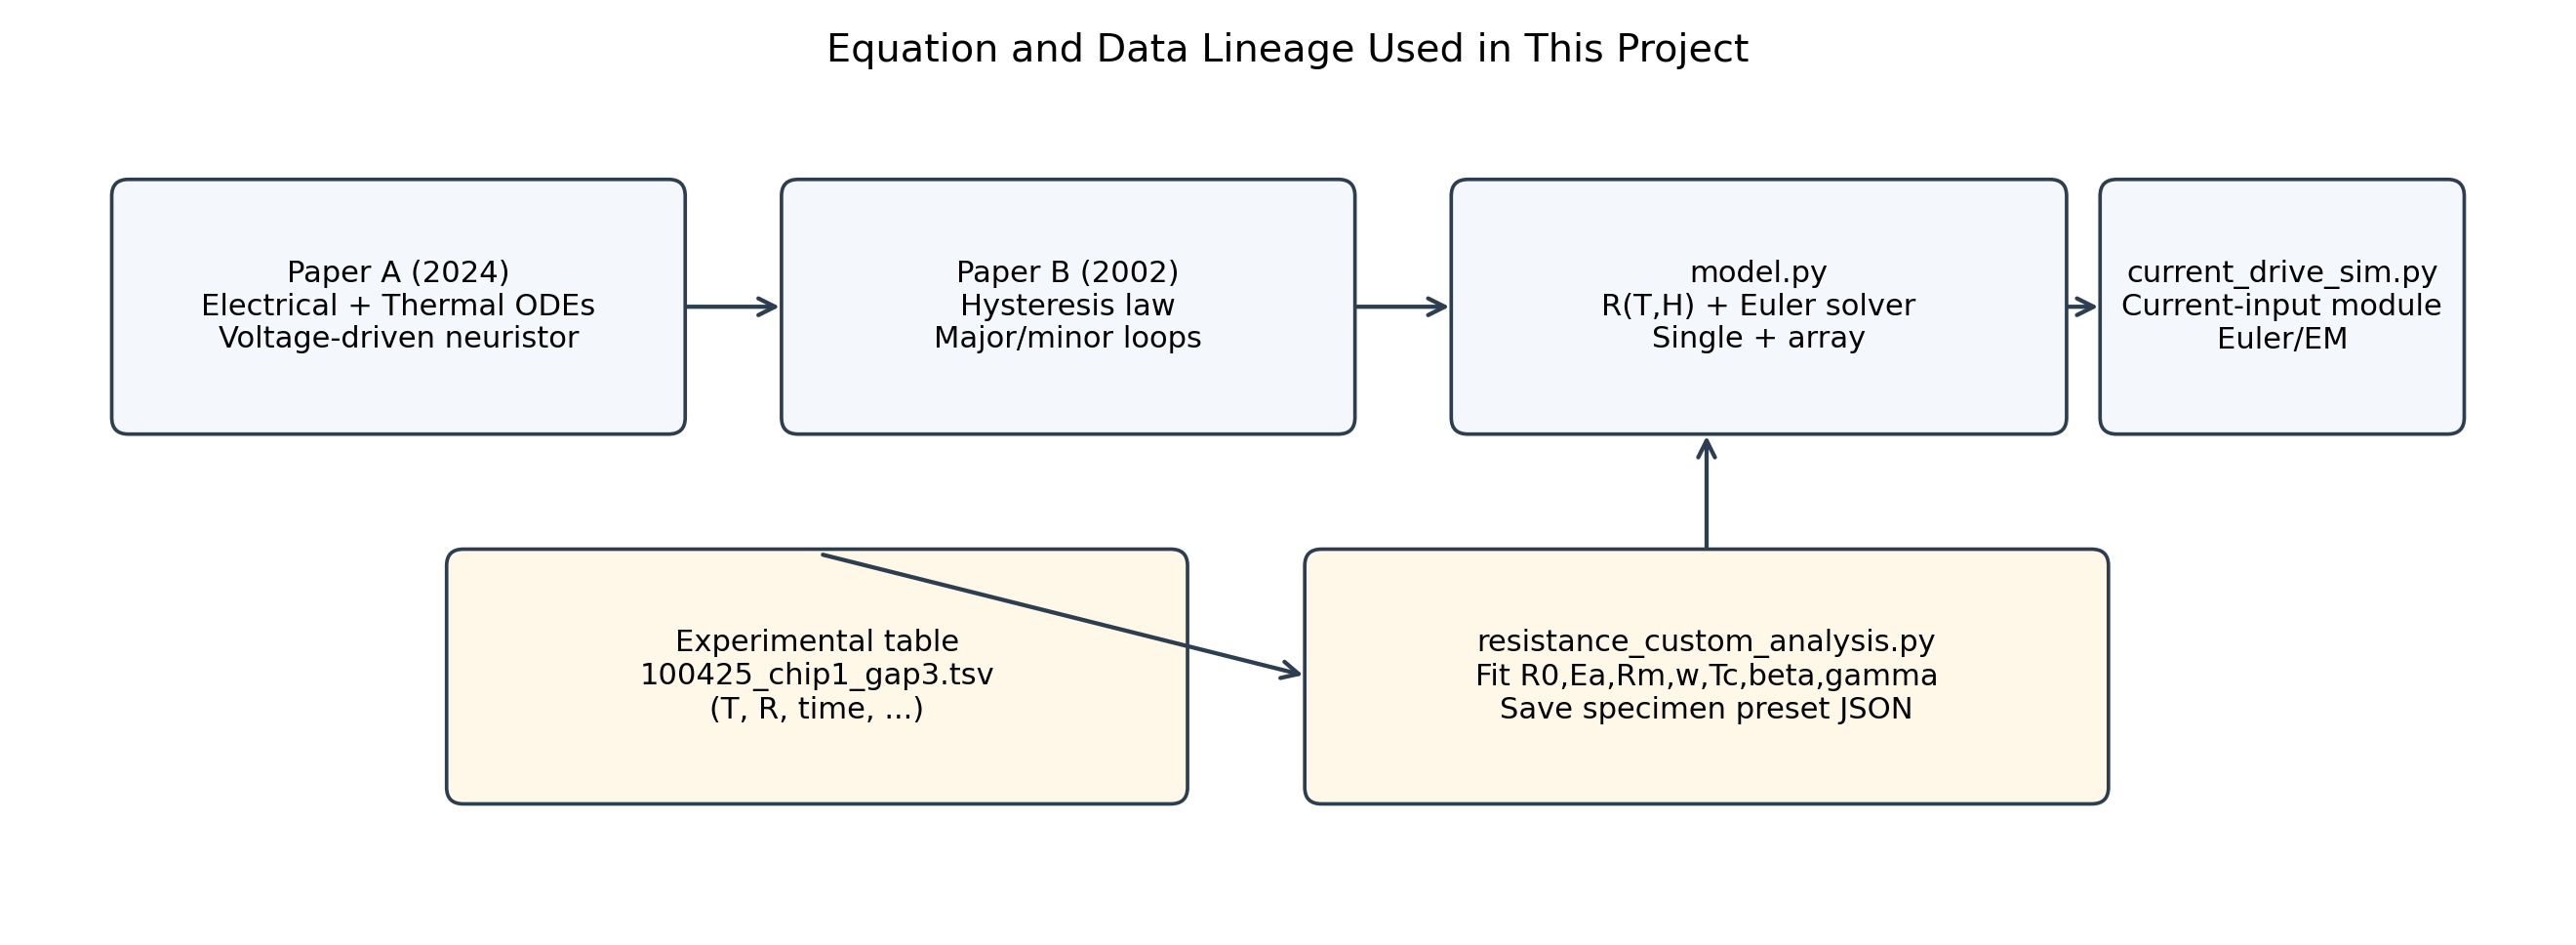
\includegraphics[width=0.98\textwidth]{outputs/paper_figures/model_lineage_flow.png}
    \caption{Equation and data lineage used in this project: papers \(\rightarrow\) model equations \(\rightarrow\) code modules \(\rightarrow\) fitted specimen parameters.}
    \label{fig:lineage}
\end{figure}

\section{Nomenclature and Units}

We define the symbols used throughout:

\begin{itemize}
    \item \(V\): device/node voltage across VO\textsubscript{2} and capacitor [V]
    \item \(V_{in}\): applied voltage source [V]
    \item \(I_{in}(t)\): injected current waveform [A]
    \item \(R_{series}\) (or \(R_{load}\)): series/load resistance [\(\Omega\)]
    \item \(R_{out}\): output/shunt resistance of current source model [\(\Omega\)]
    \item \(C\): electrical capacitance [F]
    \item \(T\): device temperature [K]
    \item \(T_0\): ambient/base temperature [K]
    \item \(C_{th}\): thermal capacitance [J/K]
    \item \(S_e\): thermal conductance to environment [W/K]
    \item \(S_c\): thermal coupling between neighboring devices [W/K]
    \item \(R(T,\mathcal{H})\): VO\textsubscript{2} resistance [\(\Omega\)], with hysteresis state \(\mathcal{H}\)
    \item \(g(T,\mathcal{H})\in[0,1]\): semiconducting fraction in hysteresis model
    \item \(R_0, E_a/k_B, R_m, w, T_c, \beta, \gamma\): hysteresis/resistance parameters
    \item \(\delta\in\{+1,-1\}\): branch indicator (heating/cooling)
    \item \((T_r,g_r,T_{pr})\): reversal-state memory variables
\end{itemize}

\section{Base Equations Taken from the Literature}

\subsection{Electrical and thermal dynamics (2024 paper)}
The reference voltage-driven neuristor equations are:
\begin{equation}
C\frac{dV_i}{dt}=\frac{V^{in}_i}{R^{load}_i}-V_i\left(\frac{1}{R_i}+\frac{1}{R^{load}_i}\right),
\label{eq:paper_electrical}
\end{equation}
\begin{equation}
C_{th}\frac{dT_i}{dt}=\frac{V_i^2}{R_i}-S_e(T_i-T_0)+S_c\nabla^2T_i+\sigma\eta_i(t).
\label{eq:paper_thermal}
\end{equation}
Equation \eqref{eq:paper_electrical} is a node-current balance (KCL) with capacitive storage, while \eqref{eq:paper_thermal} is thermal balance (Joule heating minus losses plus coupling and noise).

\subsection{Hysteretic resistance model (2002 paper lineage)}
The model form used in this project is:
\begin{equation}
R(T,\mathcal{H}) = R_0\exp\!\left(\frac{E_a/k_B}{T}\right)g(T,\mathcal{H}) + R_m.
\label{eq:R_model}
\end{equation}

Major-loop branch structure:
\begin{equation}
g = \frac{1}{2} + \frac{1}{2}\tanh\!\left[\beta\left(\delta\frac{w}{2}+T_c-(T+T_p)\right)\right].
\label{eq:g_model}
\end{equation}

Reversal-memory quantity:
\begin{equation}
T_{pr}=\delta\frac{w}{2}+T_c-\frac{1}{\beta}\operatorname{arctanh}(2g_r-1)-T_r.
\label{eq:Tpr}
\end{equation}

Proximity function used in both the paper lineage and code:
\begin{equation}
P(x)=\frac{1}{2}\left(1-\sin(\gamma x)\right)\left(1+\tanh\!\left(\pi^2-2\pi x\right)\right),
\quad
T_p = T_{pr}P\!\left(\frac{T-T_r}{T_{pr}}\right).
\label{eq:P}
\end{equation}

\section{From Paper Equations to the Implemented Voltage-Driven Model}

\subsection{Electrical equation in implemented form}
For one device, Eq.~\eqref{eq:paper_electrical} becomes
\begin{equation}
C\frac{dV}{dt}=\frac{V_{in}}{R_{series}}-V\left(\frac{1}{R(T,\mathcal{H})}+\frac{1}{R_{series}}\right),
\label{eq:V_ode_voltage}
\end{equation}
equivalently
\begin{equation}
\frac{dV}{dt}=\frac{V_{in}-V}{R_{series}C}-\frac{V}{R(T,\mathcal{H})C}.
\end{equation}

\subsection{Thermal equation in implemented form}
For one device (no spatial coupling term):
\begin{equation}
C_{th}\frac{dT}{dt}=\frac{V^2}{R(T,\mathcal{H})}-S_e(T-T_0)+\sigma\eta(t).
\label{eq:T_ode_single}
\end{equation}
For arrays, the implemented model includes \(S_c\nabla^2T\) with Neumann boundaries.

\subsection{Important implementation conventions}
\begin{itemize}
    \item Temperatures are represented in Kelvin.
    \item \(T\) is clamped to \([T_{\min},T_{\max}]\) inside hysteresis evaluation for stability.
    \item \(g\) is clipped to \([0,1]\).
    \item Unit conversions in code map user-facing \(k\Omega\), pF, and mW-based thermal units to SI before integration.
\end{itemize}

\section{Deriving the Current-Driven Module Step by Step}

\subsection{Step 1: isolate source-current contribution in voltage-drive form}
From Eq.~\eqref{eq:V_ode_voltage}, define
\begin{equation}
I_{src}\equiv \frac{V_{in}}{R_{series}}.
\end{equation}
Then
\begin{equation}
C\frac{dV}{dt}=I_{src}-V\left(\frac{1}{R(T,\mathcal{H})}+\frac{1}{R_{series}}\right).
\label{eq:intermediate_current}
\end{equation}

\subsection{Step 2: replace source with explicit current injection and finite output resistance}
Generalize \(I_{src}\to I_{in}(t)\) and \(R_{series}\to R_{out}\):
\begin{equation}
\boxed{
C\frac{dV}{dt}=I_{in}(t)-V\left(\frac{1}{R(T,\mathcal{H})}+\frac{1}{R_{out}}\right)
}
\label{eq:current_drive_main}
\end{equation}
This is exactly the electrical equation implemented in \texttt{current\_drive\_sim.py}.

\subsection{Step 3: ideal-current-source limit}
For an ideal current source:
\begin{equation}
R_{out}\to\infty \Rightarrow \frac{1}{R_{out}}\to 0,
\end{equation}
so Eq.~\eqref{eq:current_drive_main} reduces to
\begin{equation}
\boxed{
C\frac{dV}{dt}=I_{in}(t)-\frac{V}{R(T,\mathcal{H})}
}.
\label{eq:ideal_current_drive}
\end{equation}
In this project, the UI/code convention is \texttt{R\_out\_ohm <= 0} to represent this ideal limit.

\section{Discretization: Continuous Equations to Time-Stepping}

\subsection{Voltage-driven solver}
With \(t_n=n\Delta t\), explicit Euler gives
\begin{equation}
V_{n+1}=V_n+\Delta t\left[\frac{V_{in}-V_n}{R_{series}C}-\frac{V_n}{R_n C}\right],
\end{equation}
\begin{equation}
T_{n+1}=T_n+\Delta t\left[\frac{V_n^2/R_n-S_e(T_n-T_0)+S_c(\nabla^2T)_n}{C_{th}}+\text{noise}_n\right]\frac{1}{Cth\_factor},
\end{equation}
with \(R_n=R(T_n,\mathcal{H}_n)\).

\subsection{Current-driven solver}
Electrical Euler update:
\begin{equation}
V_{n+1}=V_n+\frac{\Delta t}{C}\left[I_{in,n}-V_n\left(\frac{1}{R_n}+\frac{1}{R_{out}}\right)\right].
\end{equation}

Thermal update (Euler--Maruyama form in this module):
\begin{equation}
T_{n+1}=T_n+\frac{\Delta t}{C_{th}}\left[\frac{V_n^2}{R_n}-S_e(T_n-T_0)\right]
+\frac{\sigma}{C_{th}}\sqrt{\Delta t}\,\xi_n,\quad \xi_n\sim\mathcal{N}(0,1).
\end{equation}

\section{Experimental Data to Hysteresis Inputs: Full Logic}

\subsection{Raw table extract}
Figure~\ref{fig:table_extract} shows a direct extract from the provided specimen table.

\begin{figure}[H]
    \centering
    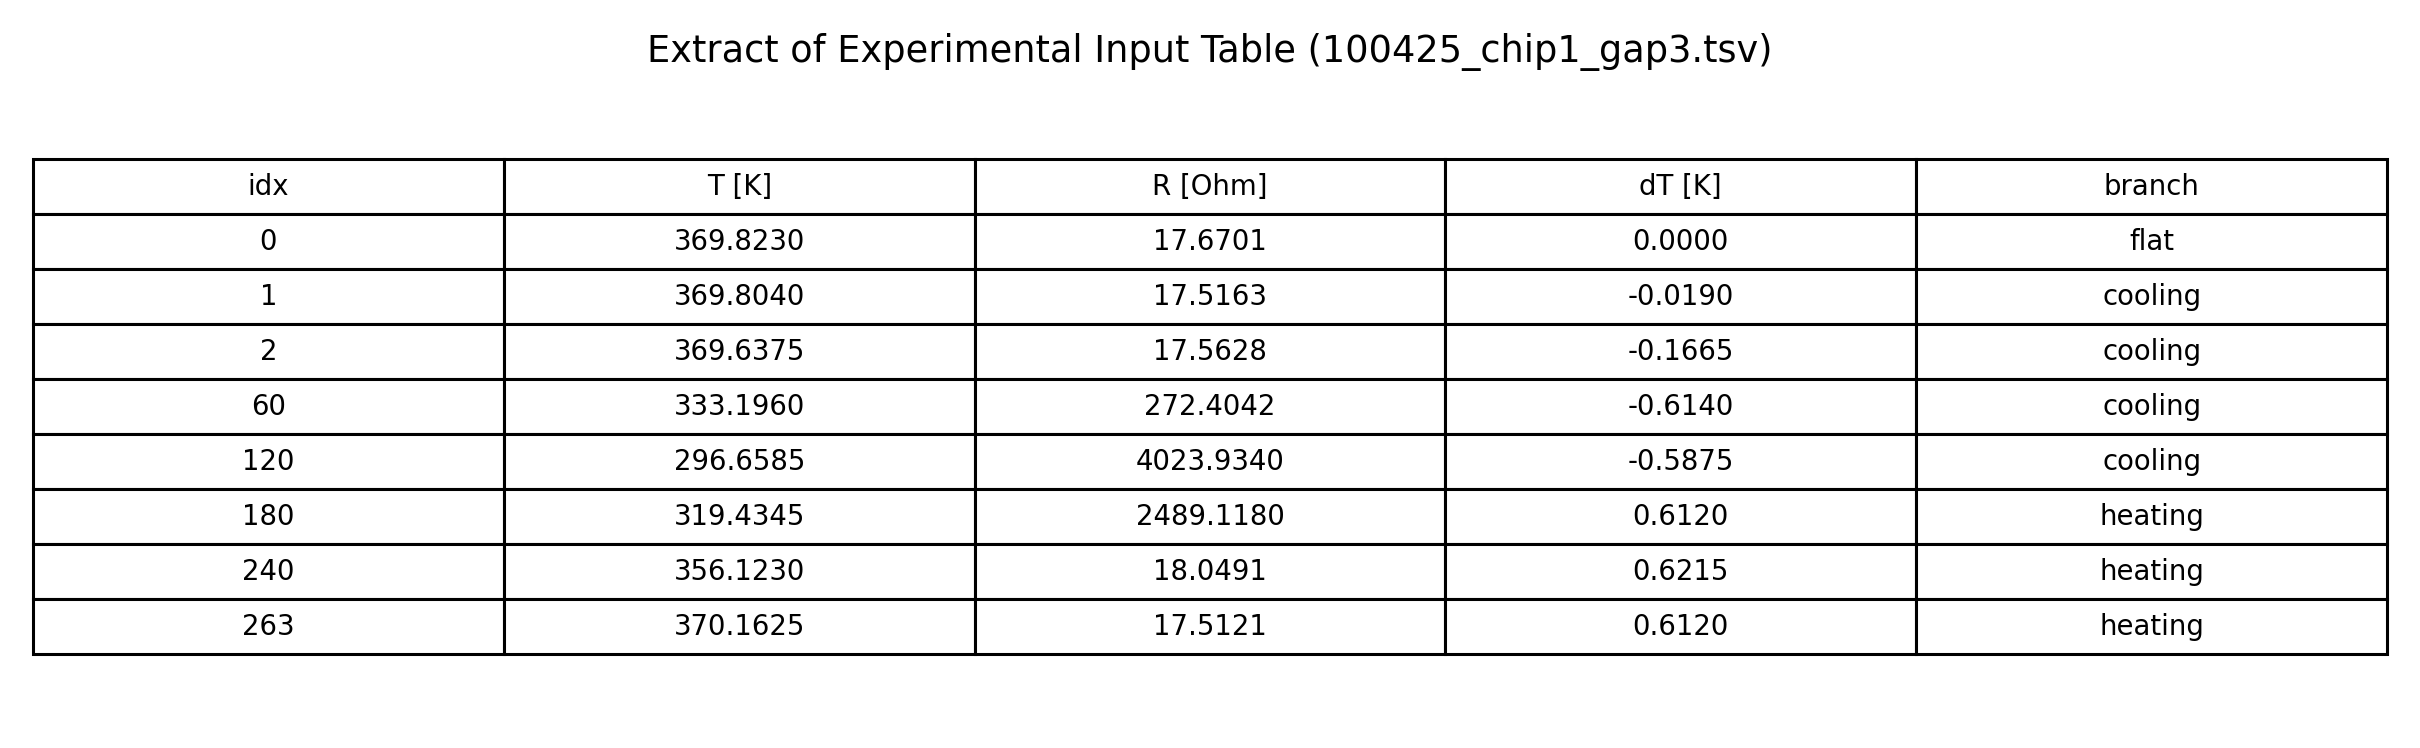
\includegraphics[width=0.95\textwidth]{outputs/paper_figures/table_extract.png}
    \caption{Extracted rows from \texttt{100425\_chip1\_gap3.tsv}. The branch label is assigned from the sign of \(\Delta T\).}
    \label{fig:table_extract}
\end{figure}

\subsection{Step A: determine branch direction from measured temperatures}
Given \(T_k\), compute
\begin{equation}
\Delta T_k = T_k - T_{k-1}.
\end{equation}
Then:
\[
\Delta T_k>0 \Rightarrow \text{heating}, \qquad
\Delta T_k<0 \Rightarrow \text{cooling}.
\]
This branch information is crucial because the hysteresis model is path-dependent.

\subsection{Step B: build seed estimates for \(R_0, E_a, R_m\)}
Using low-temperature points (where semiconducting behavior dominates), we scan candidate \(R_m\) values and linearize:
\begin{equation}
\ln(R-R_m)=\ln R_0+\frac{E_a}{T}.
\label{eq:arrhenius_linear}
\end{equation}
For each \(R_m\) candidate, linear regression on Eq.~\eqref{eq:arrhenius_linear} gives a slope/intercept pair \((E_a,\ln R_0)\). The candidate with smallest regression error is used as seed.

\subsection{Step C: convert measured \(R(T)\) into a seed \(g(T)\)}
From Eq.~\eqref{eq:R_model}, algebraic inversion yields:
\begin{equation}
g_{\text{seed}}(T)=
\frac{R(T)-R_m^{\text{seed}}}{R_0^{\text{seed}}\exp(E_a^{\text{seed}}/T)},
\end{equation}
followed by clipping to \([0,1]\).

\subsection{Worked numerical example (actual row from the dataset)}
Using one measured row (\(T=\) 319.4345 K, \(R=\) 2489.118 \(\Omega\)) and one seed triplet estimated from the dataset (\(R_0^{\text{seed}}=10.9606\ \Omega\), \(E_a^{\text{seed}}=1753.57\ \text{K}\), \(R_m^{\text{seed}}=0.8688\ \Omega\)):
\begin{align}
\text{denominator} &= R_0^{\text{seed}}\exp(E_a^{\text{seed}}/T)
= 10.9606\cdot \exp(1753.57/319.4345) \\
&\approx 2654.226,\\
g_{\text{seed}} &= \frac{2489.118-0.8688}{2654.226} \approx 0.93747.
\end{align}
This demonstrates exactly how measured \(R,T\) points are transformed into a hysteresis-related quantity used in fitting.

\subsection{Pipeline visualization}
\begin{figure}[H]
    \centering
    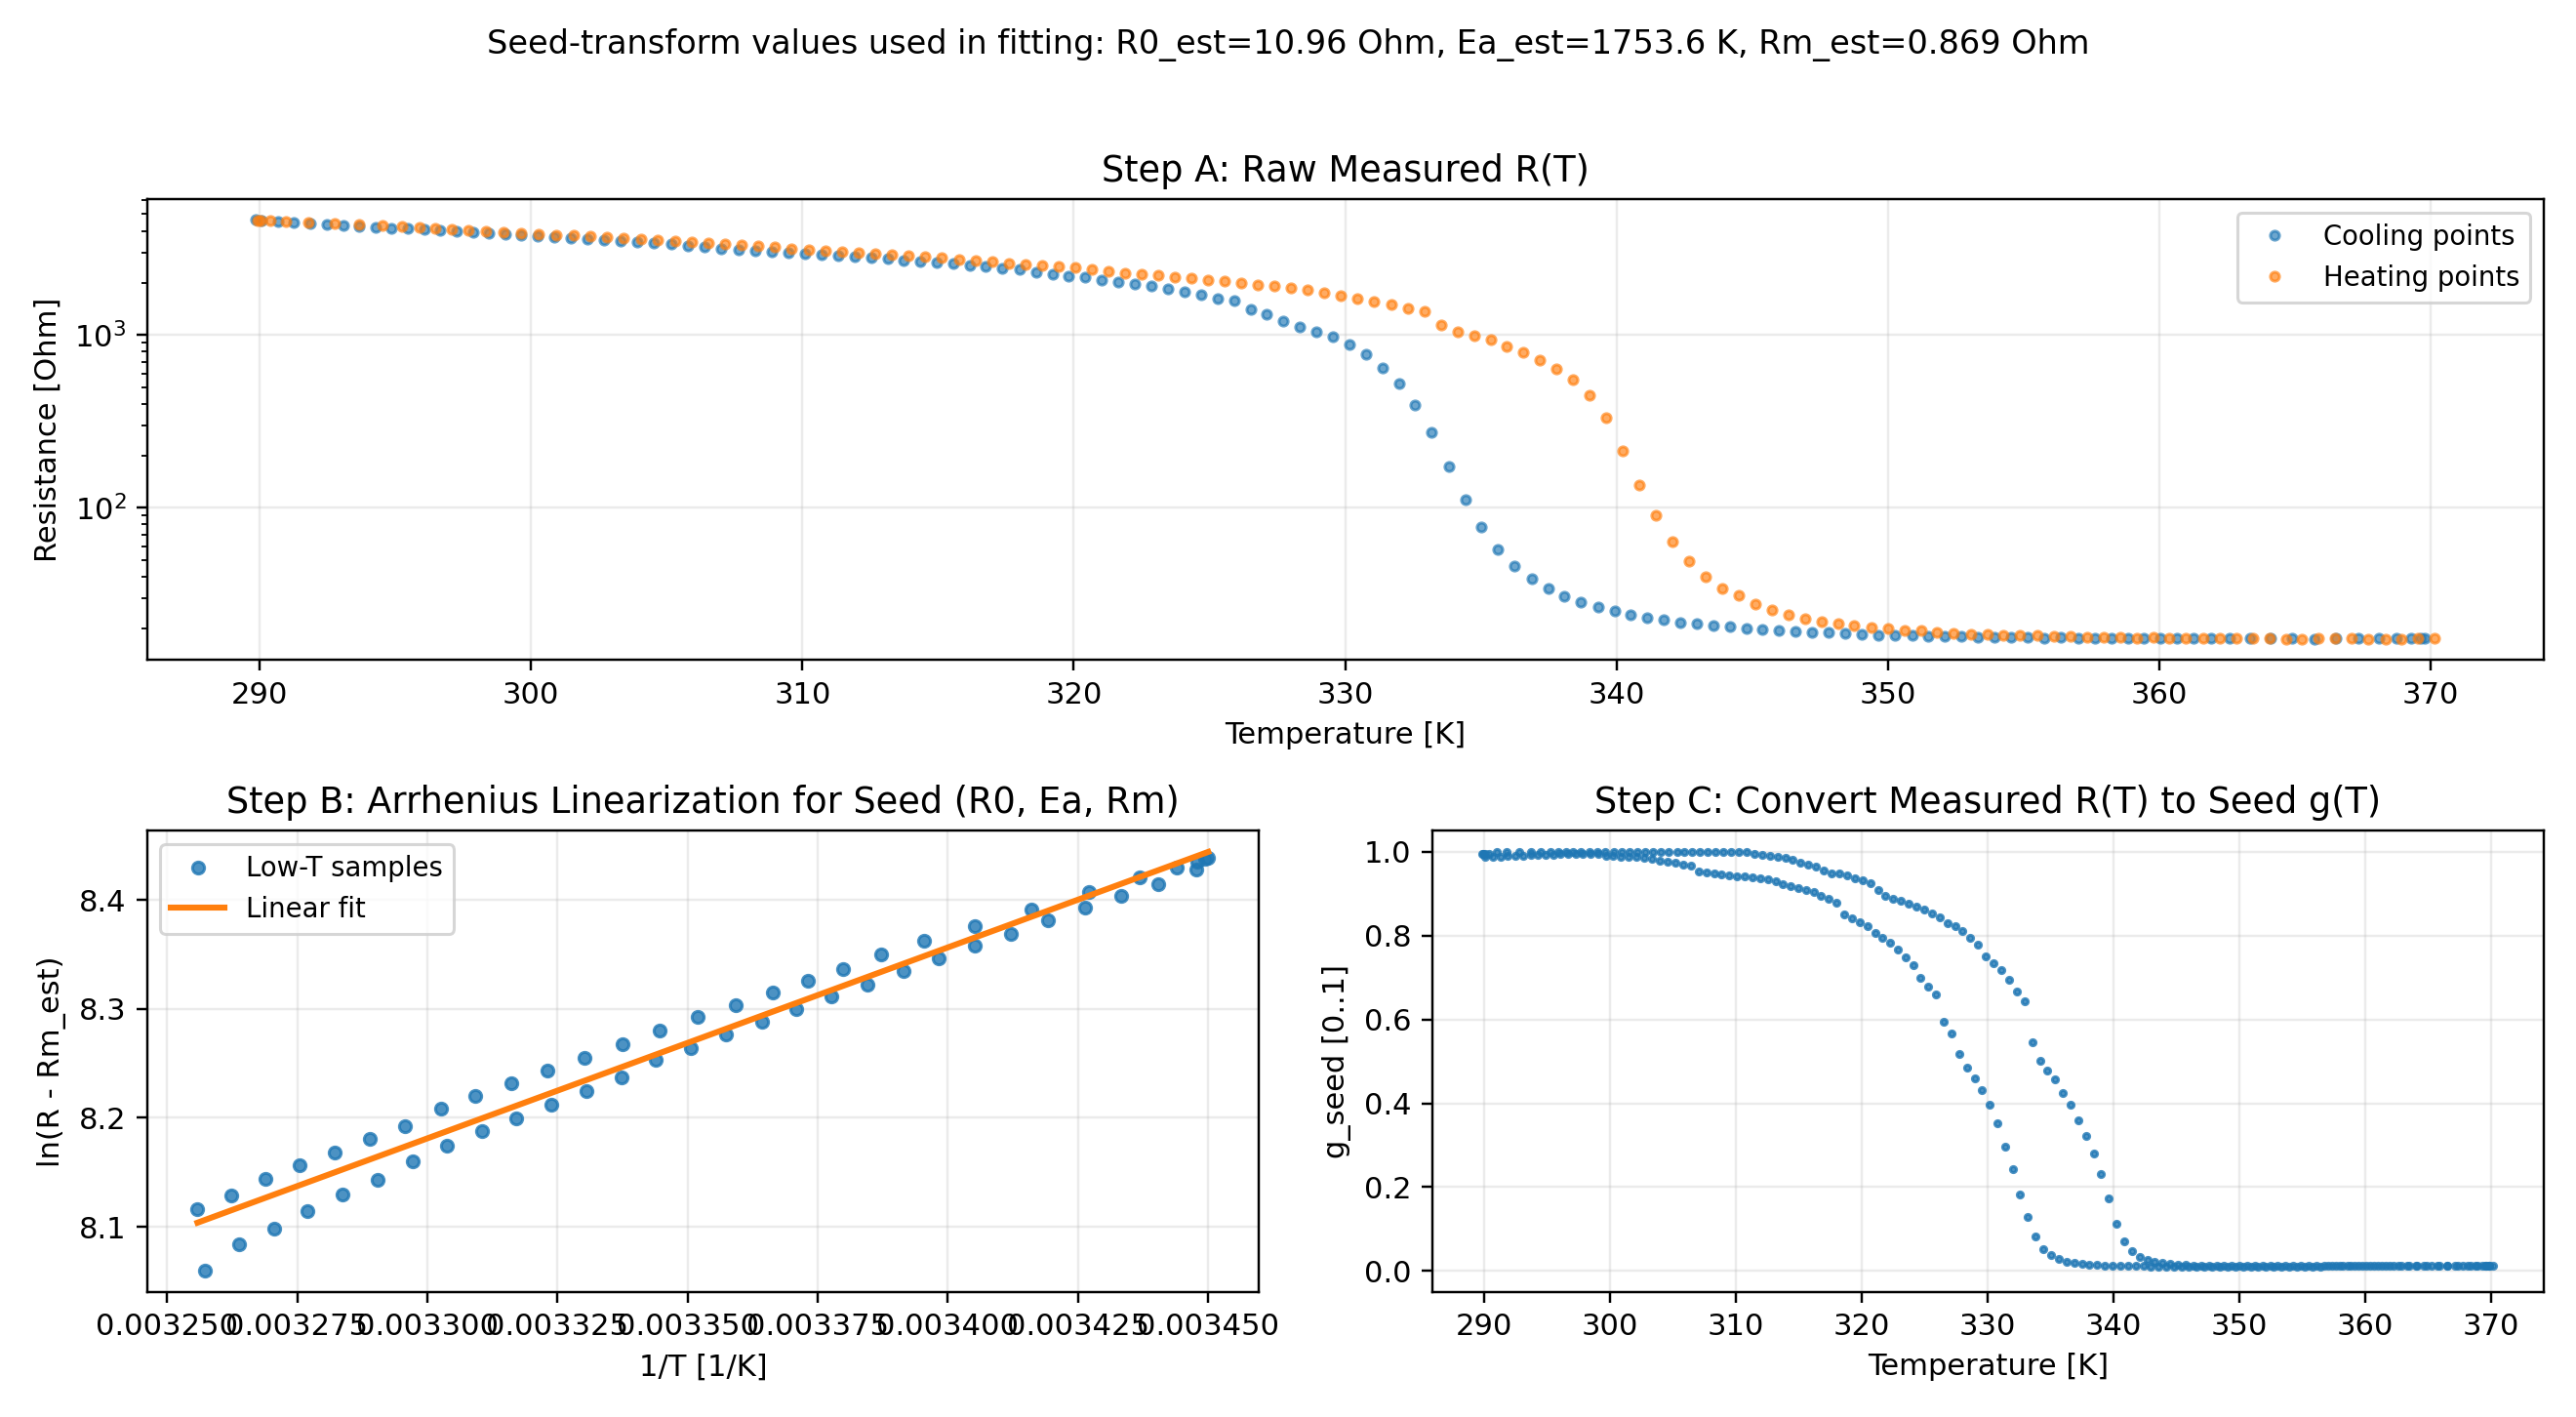
\includegraphics[width=0.98\textwidth]{outputs/paper_figures/fit_transform_pipeline.png}
    \caption{Didactic pipeline: (A) raw \(R(T)\), (B) Arrhenius linearization for seed extraction, (C) transformed seed \(g(T)\).}
    \label{fig:transform_pipeline}
\end{figure}

\section{How the Fit is Performed in Code}

\subsection{Model being fitted}
The fitter uses the \emph{same} hysteresis evaluator used by simulation (shared physics, not a separate ad-hoc curve).

\subsection{Objective}
The fitting objective combines resistance fidelity and consistency of transformed \(g\):
\begin{equation}
\mathcal{J}=
\mathrm{RMSE}_{\log_{10}}(R_{\text{pred}},R_{\text{meas}})
+\lambda\,\mathrm{RMSE}(g_{\text{pred}},g_{\text{exp}})
+\text{(small optional penalty)},
\end{equation}
with \(\lambda=\texttt{g\_weight}\).

\subsection{Search strategy}
\begin{enumerate}
    \item Seed from paper-default and data-derived candidates.
    \item Random search for global exploration.
    \item Coordinate-descent local refinement.
    \item Branch check (\texttt{insulator} vs \texttt{metal}) and keep lower-loss solution.
\end{enumerate}

\section{Fitted Model Results (Specimen 100425\_chip1\_gap3)}

\subsection{Saved fit metrics}
From \texttt{presets/resistance\_100425\_chip1\_gap3.json}:
\begin{itemize}
    \item \(\mathrm{RMSE}_{\log_{10}}(\text{overall})=0.03756\)
    \item \(\mathrm{RMSE}_{\log_{10}}(\text{cooling})=0.03432\)
    \item \(\mathrm{RMSE}_{\log_{10}}(\text{heating})=0.04067\)
    \item selected initial branch: \texttt{metal}
\end{itemize}

\subsection{Fitted parameter set}
\begin{table}[H]
\centering
\caption{Fitted resistance/hysteresis parameters stored in project preset JSON.}
\begin{tabular}{>{\raggedright\arraybackslash}p{0.32\textwidth} p{0.22\textwidth} p{0.34\textwidth}}
\toprule
Parameter & Value & Meaning \\
\midrule
\(R_0\) & 0.5297359 \(\Omega\) & Arrhenius prefactor \\
\(E_a/k_B\) & 2658.023 K & Activation term in Kelvin form \\
\(R_{m0}\) & 18.19784 \(\Omega\) & Metallic base resistance \\
\(R_m\text{ factor}\) & 1.0 & Metallic scaling factor \\
\(w\) & 6.90033 K & Hysteresis width \\
\(T_c\) & 333.5702 K & Hysteresis center \\
\(\beta\) & 0.2969915 K\(^{-1}\) & Branch steepness \\
\(\gamma\) & 0.9562697 & Proximity window parameter \\
Reversal threshold & 0.01 K & Minimal \(|\Delta T|\) for branch reversal \\
\bottomrule
\end{tabular}
\label{tab:fitted_params}
\end{table}

\subsection{Overlay against measured data}
\begin{figure}[H]
    \centering
    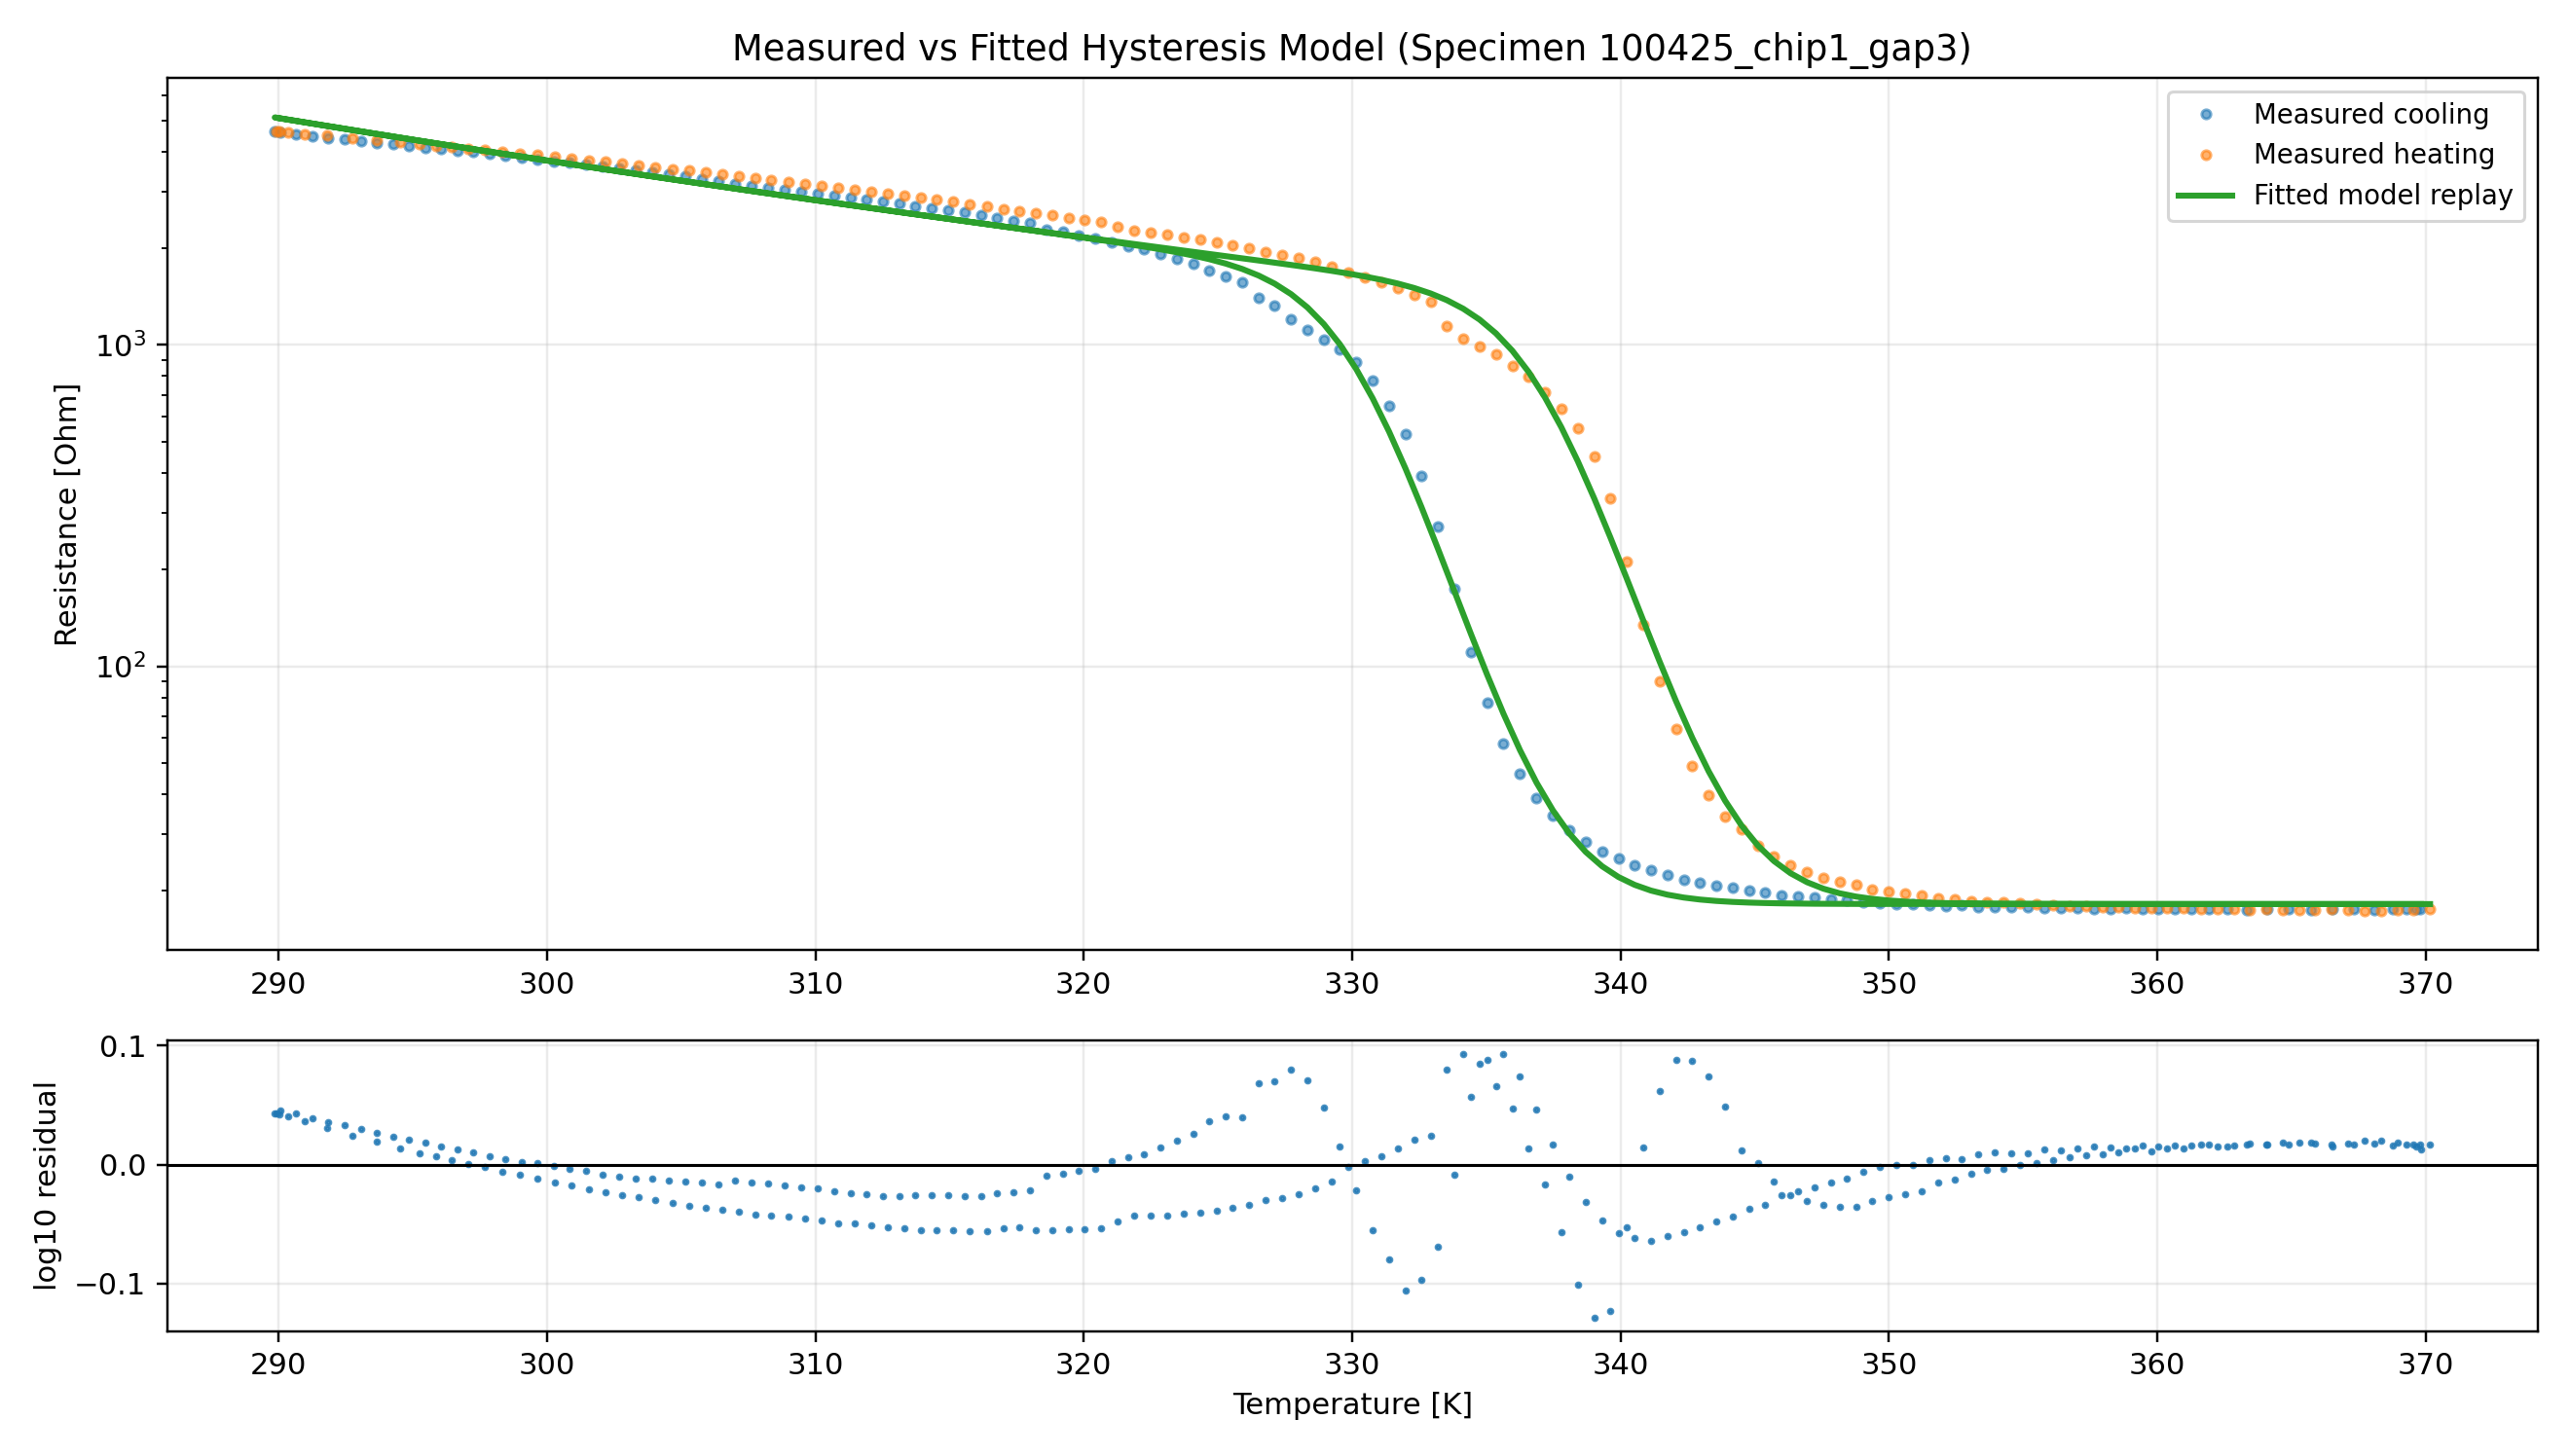
\includegraphics[width=0.98\textwidth]{outputs/paper_figures/fit_overlay_with_residuals.png}
    \caption{Measured points versus fitted model replay, with residuals in \(\log_{10}\) space.}
    \label{fig:fit_overlay}
\end{figure}

\section{What the Simulators Do, Algorithmically}

\subsection{Voltage-driven simulation loop (\texttt{model.py})}
At each step:
\begin{enumerate}
    \item Evaluate \(R_n,g_n\) from \(T_n\) and hysteresis state.
    \item Compute electrical derivative from Eq.~\eqref{eq:V_ode_voltage}.
    \item Compute thermal derivative from Eq.~\eqref{eq:T_ode_single} (plus optional coupling/noise).
    \item Euler-update \(V_{n+1},T_{n+1}\).
    \item Update and store traces \((V,I_{load},I_{vo2},T,R,g)\).
\end{enumerate}

\subsection{Current-driven simulation loop (\texttt{current\_drive\_sim.py})}
At each step:
\begin{enumerate}
    \item Read \(I_{in,n}\) from pulse/step waveform.
    \item Evaluate \(R_n\) from hysteresis at \(T_n\).
    \item Update \(V_{n+1}\) via Eq.~\eqref{eq:current_drive_main}.
    \item Update \(T_{n+1}\) via deterministic thermal term plus optional stochastic increment.
    \item Update hysteresis reversal memory with \((T_n,T_{n+1})\).
\end{enumerate}

\section{Reproducibility Artifacts}

This manuscript is paired with generated figures located at:
\begin{itemize}
    \item \texttt{outputs/paper\_figures/model\_lineage\_flow.png}
    \item \texttt{outputs/paper\_figures/table\_extract.png}
    \item \texttt{outputs/paper\_figures/fit\_transform\_pipeline.png}
    \item \texttt{outputs/paper\_figures/fit\_overlay\_with\_residuals.png}
\end{itemize}

Figure generation command:
\begin{verbatim}
python scripts/generate_paper_figures.py
\end{verbatim}

Core files used for this derivation:
\begin{itemize}
    \item \texttt{model.py}
    \item \texttt{current\_drive\_sim.py}
    \item \texttt{resistance\_custom\_analysis.py}
    \item \texttt{app.py}
    \item \texttt{data/experimental/100425\_chip1\_gap3.tsv}
    \item \texttt{presets/resistance\_100425\_chip1\_gap3.json}
\end{itemize}

\section{Conclusion}

The implemented project model is not an ad-hoc black box: it is a direct computational realization of (i) the thermal-neuristor ODE framework from the 2024 paper and (ii) the hysteretic VO\textsubscript{2} resistance model lineage from the 2002 paper, with specimen-level calibration from measured \(R(T)\) data. The current-driven module follows from explicit source transformation and a clearly defined ideal-source limit. The full pipeline from measured table rows to fitted parameters is reproducible, equation-by-equation, and supported by generated diagnostic figures.

\begin{thebibliography}{9}
\bibitem{zhang2024}
Y.-H. Zhang, C. Sipling, E. Qiu, I. K. Schuller, and M. Di Ventra,
``Collective dynamics and long-range order in thermal neuristor networks,''
\emph{Nature Communications}, vol. 15, 6986, 2024.

\bibitem{almeida2002}
L. A. L. de Almeida, G. S. Deep, A. M. N. Lima, and H. Neff,
``Modeling of the hysteretic metal-insulator transition in a vanadium dioxide infrared detector,''
\emph{Optical Engineering}, vol. 41, no. 10, pp. 2582--2588, 2002.
\end{thebibliography}

\end{document}
